\chapter{Visualization Methods}
\label{Chapter2}

%------------------------------------------------------------------------------

\section{Viewing Volume, Viewing Frustum, Viewing Field, and Visualization Requirements}
\label{VisualizationRequirements}

In natural sense, viewing volume of a camera is defined by an infinite half cone, apex of which corresponds to the focal point of the camera. Because real computers cannot have unlimited resources, in practical computer 3D technology we usually limit the bottom of the cone by a far clip plane, then limit the top of the cone even more by a near clip plane, and express the result by a frustum (figure \ref{fig:ViewingVolume}). To visualize the viewing volume, there may be many methods other than directly rendering the volume. Thus in this research we abstract the viewing volume by the term ``viewing field''.

\begin{figure}[htbp]
	\centering
	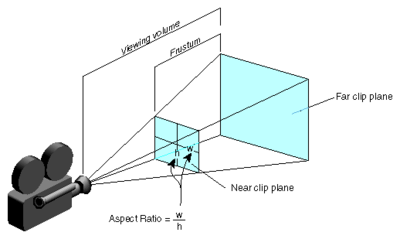
\includegraphics{./Primitives/viewing_volume.png}
	\rule{35em}{0.5pt}
	\caption[Viewing volume of camera]{Viewing volume of camera}
	\label{fig:ViewingVolume}
\end{figure}

There may be many visualization methods, not limited to the ones discussed in the next section. But for a method to find practical use in outdoor MR, it should be able to be implemented (see section \ref{UseCases} to have a rough illustration) so that it meets the following basic qualitative requirements, expressed in the ``it should'' tongue of most DSLs (Domain Specific Language) of the BDD (Behavior Driven Development) methodology in software engineering:

\begin{itemize}
	\item It should be easy for the user to understand when they see the visualized viewing fields of surrounding surveillance cameras.
	\item It should work in realtime. When the user changes the position or orientation of the mobile device, the video displayed on the screen of the mobile device should simultaneously change accordingly to the movement without much delay.
	\item It should have good accuracy. In order to correctly overlay CG objects onto the original video, the position and orientation of the mobile device's camera must be estimated within a small error.
	\item It should be robust to disturbance in outdoor environment. In outdoor environment, naturally there may be many passers-by and they may prevent the mobile device's camera from continuously capturing a scene. If the system use GPS device, the GPS signal strength may change a lot when the user walk from an open space to a space shadowed by trees or buildings.
\end{itemize}

When implementing the prototype in chapter \ref{Chapter3} and conducting experiment to evaluate the visualization methods, we must take the above requirements into account.

%------------------------------------------------------------------------------

\section{Visualization Methods}
\label{VisualizationMethods}

% In this section, we propose five methods to visualize viewing fields of . This section discusses the idea and algorithm of the methods. Based on this discussion, chapter \ref{Chapter3} will implement and integrate these methods into a working prototype.
% 
% \subsection{Volume Method}
% 
% As discussed above, the natural method to visualize the viewing field is thus simply visualizing this volume (figure \ref{fig:VolumeMethod}). However, the volume usually occupies all the scene viewed from the mobile camera, especially if the user is inside the viewing volume. The visualization produced by this method is hard to understand.
% 
% \begin{figure}[htbp]
% 	\centering
% 	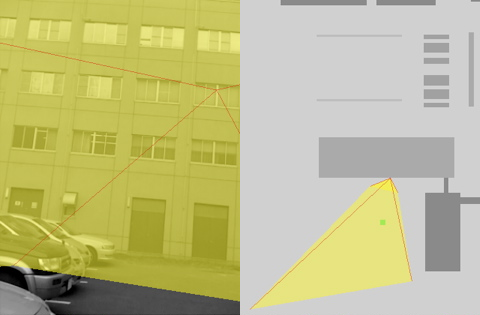
\includegraphics{./Primitives/theory_volume.png}
% 	\rule{35em}{0.5pt}
% 	\caption[Volume Method]{Volume Method}
% 	\label{fig:VolumeMethod}
% \end{figure}
% 
% \subsection{Shadow Method}
% 
% The fact that the frame captured by the camera is perspective projection of the volume into the near plane of the frustum gives us another method. This method visualizes the virtual shadow created by the light positioned at the eye-point of the camera and the near plane of the frustum (figure \ref{fig:ShadowMethod}). This method gives more understandable visualization. There are various ways to render the shadow, the two popular ones are shadow mapping \cite{Reference7} \cite{Reference8} and volume shadow \cite{Reference9}.
% 
% \begin{figure}[htbp]
% 	\centering
% 	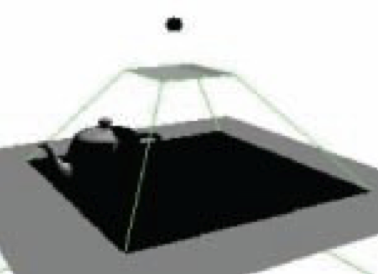
\includegraphics{./Primitives/theory_shadow.png}
% 	\rule{35em}{0.5pt}
% 	\caption[Shadow Method]{Shadow Method}
% 	\label{fig:ShadowMethod}
% \end{figure}
% 
% \subsection{Contour Method}
% 
% An alternative method is to only visualize the contours of the shadow (figure \ref{fig:ContourMethod}). Rendering only the contour is much lighter than rendering the whole shadow, thus this method is supposed to be much faster.
% 
% \begin{figure}[htbp]
% 	\centering
% 	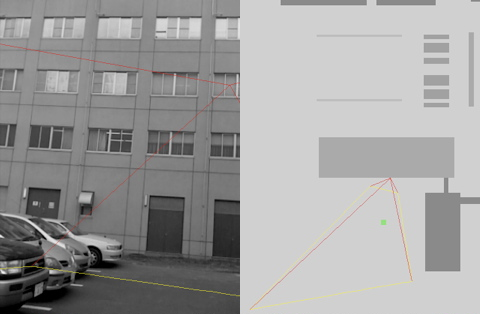
\includegraphics{./Primitives/theory_contour.png}
% 	\rule{35em}{0.5pt}
% 	\caption[Contour Method]{Contour Method}
% 	\label{fig:ContourMethod}
% \end{figure}
% 
% \subsection{Vector Method}
% 
% For most of the time, a person may want to know not only the viewing field, but also the position and distance to the surveillance camera, To visualize this information, we propose a method using vectors (figure \ref{fig:VectorMethod}). In the figure, all the vectors are pointing the camera, and the length of the vectors are reverse proportional to the distance from the root of the vectors to the camera.
% 
% \begin{figure}[htbp]
% 	\centering
% 	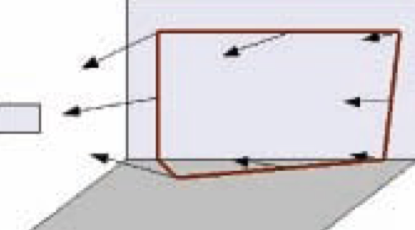
\includegraphics{./Primitives/theory_vector.png}
% 	\rule{35em}{0.5pt}
% 	\caption[Vector Method]{Vector Method}
% 	\label{fig:VectorMethod}
% \end{figure}
% 
% \subsection{Animation Method}
% 
% We are studying the visualization method in which animate objects coming from the surveillance cameras are used to visualize the viewing fields. This method has  many advantages:
% 
% \begin{itemize}
% 	\item The moving objects start form the surveillance camera positions, as a result the user easily knows the camera positions.
% 	\item Event when the mobile camera is fixed at a certain position and orientation, the visualization effect is still achieved.
% 	\item The moving objects do not block the scene, as a result the user can see the scene and visualized camera viewing fields at the same time.
% \end{itemize}
% 
% \begin{figure}[htbp]
% 	\centering
% 	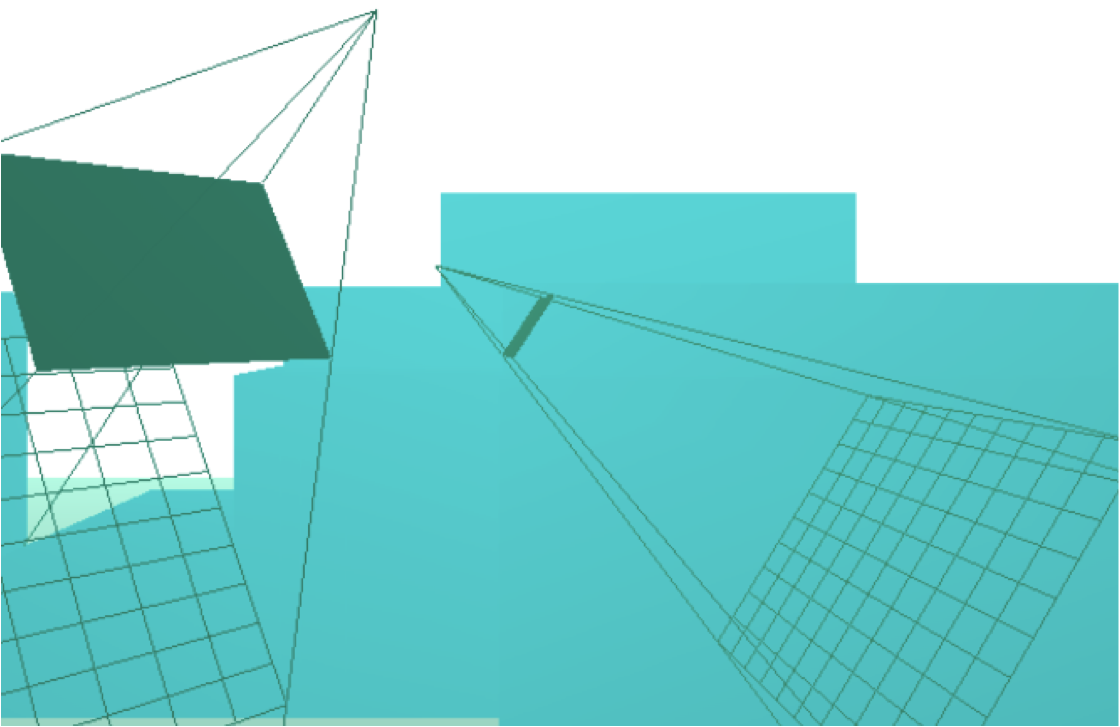
\includegraphics{./Primitives/theory_animation.png}
% 	\rule{35em}{0.5pt}
% 	\caption[Animation Method]{Animation Method}
% 	\label{fig:AnimationMethod}
% \end{figure}
